So far we have covered how import session types can describe communication protocols and allow processes to exchange runtime through import tokens.
In this section, we come back to UC and illustrate how NomosUC can be used to realize any any arbitrary configuration of ITMs in UC by proposing an abstract channel design, called \emph{providerless channels}, that overcome a communication limitation of binary session types.
Next, we cover how NomosUC can support an arbitrary number of parties by using sandboxing and providerless channels. 
Finally, we describe how a simulator is constructed in NomosUC, and the composition operators that we realize.

%So far we have introduced a type system and process calculus for writing and checking runtime that conforms to the import mechanism for polynomial time.
%In this section, we show how NomosUC processes overcome a limitation of binary session types to realize any arbitrary configuration of ITMs, and describe how \emph{providerless channels} and sandboxing enable an arbitrary number of protocol parties. 
%Next, we realize the Dummy Lemma (sometimes described as completeness of the dummy adversary~\cite{gnuc}), an important result in used as a standard result intended to show the expressiveness of new UC programming tools or formulations~\cite{ilc,easyuc,gnuc}.
%Despite the machinery required to realize import, our approach yields a surprisingly simple simulator proof.
%Finally, we realize UC composition by first realizing a simpler composition operator~\cite{ilc}, a multisession theorem with join state~\cite{symbolicuc,juc}, and combine them in a natural way to state the full composition theorem in NomosUC.

\subsection{Capturing the UC Computation Model}
An extreme limitation of binary session types is the communication topologies that they can realize.
When a linear channel is created, it is offered by a process called the ``provider'' and given to a process called the ``client'', and impose a strict parent-child relationship between processes.
The process configuration in Figure~\ref{fig:pandq} is not realizable, because of the circular dependency. 
$P$ must be spawned by $Q$, giving $Q$ its channel, and $Q$ must be spawned by $P$ in order to give it its channel.
We overcome this limitation by using shared session types to create a new abstract channel called a \emph{providerless channel}.
Shared channels allow us to define a message buffer called a communictor, that lets multiple other processes use its channel and use it to send messages.
The communicator can be thought of as a message buffer, and any process can attempt to \emph{acquire} its channel, check for new messages with \mb{poll}, and place another message in the bugger with \m{push}.
The session type of the communicator is given below, along with operators to acquire ($\up$) and release ($\down$) operators, below, and the full typing rules of shared session types is given in Appendix~\ref{app:typing_rules}.
We provide the full typing rule of shared session types and the communicator in the Appendix.

Communicators introduce some constraints. 
First its session type is simple and only allows adding a messages and polling for a new message.
This means that messages sent over it are functionally typed and enforce no message ordering of their own.
Second, only a constant amount of import can be sent through the communicator because it only has one possible label, $\mb{push}$.
We overcome these limitations, for the type system and for the programmer's experience, through the abstract channel shown in Figure~\ref{fig:newpandq}.
Rather than $P$ and $Q$ offering each other their channels, new dummy processes are created ($a_p, b_p, a_q, b_q$) that offer both $P$ and $Q$ the session types that they expect, \m{PtoQ} and \m{QtoP}.
These process communicate and translate messages from $C$ to the corresponding label on on the channels they offer, and vice verssa.
The triviality of these dummy processes, means their code can be easily generated as one long case statement.
\emph{The programmer need only specify the session type, the functional message type, and a mapping between them.}

\todo{the processes $P$ and $Q$ are virtualized, make a precise statement more concise of what happens}
We refer the reader to Appendix~\ref{app:itm} for an example of what the generated code for a providerless channel looks like for our running commitment example, an example of a cyclic topology of processes and how it is realized by providerless channels, and an an argument of why we can use this construction to realized any arbitrary ITM topology as a process configuration.

\vspace{-1mm}
{\centering
\scalebox{0.9}{
\parbox{0cm}{
\begin{tabbing}
$\m{comm[\tau]\{n\}} = \up \echoice{$\=$ \textcolor{red}{\getpot^n} \mb{push}: \m{\tau} \arrow \m \down \m{comm[\tau]},$\\
\>$\textcolor{red}{\getpot^0} \mb{poll}: \ichoice{$\=$\textcolor{red}{\paypot^{n}} \mb{yes}: \m{\tau} \;\product \down \m{comm[\tau]},$\\
\>\>$\textcolor{red}{\paypot^0} \mb{no}: \; \down \m{comm[\tau]}}}$
\end{tabbing}}}
\par}

%The new constructors $\up$ and $\down$ indicate an acquire-release paradigm to prevent non-determinism, along with the write token, when both $P$ or $Q$ attempt to write.
%A sender $P$ acquires the communicator's channel, $\#c$, and $\mb{push}$es a functionally 
%typed message along with some import $\textcolor{red}{\getpot^n}$.
%The receiver $Q$ waits for $\#c$ to be released and asks for a new message with $\mb{poll}$. 
%If a new message was written, $Q$ receives label $\mb{yes}$ on $\#c$, the message, and the import.
%Otherwise the channel takes the $\mb{no}$ branch.
%We provide the full typing rule of shared session types in Appendix~\ref{app:typing_rules}.
\begin{figure}
    \begin{subfigure}{0.5\textwidth}
    \begin{center}
    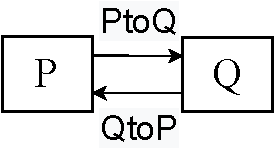
\includegraphics[scale=0.5]{figures/p_and_q.pdf}
    \caption{ITMs can communicate like this. NomosUC processes can't offer their channels to each other.}
    \label{fig:pandq}
    \end{center}
    \vspace{1em}
    \end{subfigure}
    \begin{subfigure}{0.5\textwidth}
    \begin{center}
    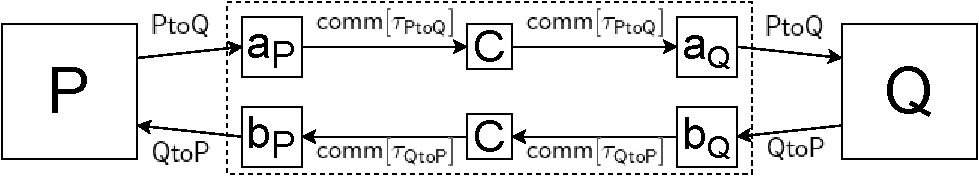
\includegraphics[scale=0.4]{figures/newPandQ.pdf}
    \caption{Processes that make up providerless channels.}
    \label{fig:newpandq}
    \end{center}
    \vspace{0.5em}
    \end{subfigure}
    \caption{Channels are labeled with their types.}
\end{figure}

\plan{Right here was a more in depth about providerless channel constructions and how the different processes are spawned, but we move that to the appendix. Describing it here concisely only makes it more confusing rather than less. In the appendix they can be presented with a full descriptive example of a cycle of three ITMs.}
%Communicators alone, however, would constraint all processes in NomosUC to communicate through the same type $\m{comm[m]\{n\}}$, negating the descriptive session types we want from using session types.
%
%We abstract channels into \emph{providerless channels}: a channel implemented by a communicator and some dummy processes whose code is generated at compile-time.
%In Figure~\ref{fig:newpandq}, we show an illustration of a providerless channel. The dummy processes $a_P$ and $b_P$ offer the linear session types that $P$ expects and communicates with $Q$ through the communicator.
%Process $a_P$ case matches on the labels in type \m{PtoQ} and sends the analogous, functionally-typed $\tau_{\m{PtoQ}}$ message to the communicator, and vice-versa for receiving from \m{C}.
%For example for \Fdb and a party (in relation to Figure~\ref{fig:newpandq}), $\m{QtoP} := \m{db}[k][v]$ and $\tau_\m{QtoP} :=$ Store \inline{of PID k v |} OK \inline{of PID |} Get \inline{of PID k |} Yes \inline{of v |} No.
%
%Spawning the processes in a providerless channel must be done in a specific order given the linearity of the channels that $a_P$ and $b_P$ offer. 
%The communicator, $C$, is spawned first. The party $P$ must be a client of $a_P$ and $b_P$ and, therefore, its initialization code spawns them first, gives them the shared  $\#c$, and begins communication.  
%In general, every process using providerless channels must have initialization code like this. 
%The intitialization is trivial and the dummy processes simple case statements.
%\emph{Therefore, generating their code at compile-time given the only the relevant types relieves a big burden on the programmer.}
%We given an example of a NomosUC process, it's session types, and show what $a_P$, $b_P$, and the wrapped process look like in Appendix~\ref{app:expand}.
%In Appendix~\ref{app:itm} we use prodiverless channels to show that \emph{NomosUC processes can realize any ITM system and vice versa (NomoUC $C' \Leftrightarrow$ ITMs $M'$)}.

%A important consequence of providerless channels is that the session type of communicators accepts a \emph{constant} amount of import on every message.
%It means that in addition to specifying $\tau_\m{PtoQ}$ the user must also specify the constant import parameter given to the providerless channel.
%For example for a session type with two labels, one sending $n$ import and one $m$, the communicator in the providerless channel is parameterized with \emph{at least} $max(n,m)$ import to ensure sufficient runtime.
%In general, this doesn't restrict what NomosUC can realize but does mean the programmer must take care when setting import values for protocols and functionalities.
%Fortunately, this doesn't affect the Theorems we prove in this section as they are agnostic of the types of the processes they use.
%Furthermore, precise runtime constraints or reasoning about efficient algorithms is not an intended goal of UC, and functionality and protocol code are still written according to the more descriptive session types they use.

%\paragraph{\textbf{Dynamic Parties and Functionalities}}
\subsection{Dynamic Parties and Functionalities}
Prior works that create security proofs or attempt some form of UC runtime analysis only do so for a statically defined number of instances of a protocol or functionality, \cite{ilc,ipdl,easyuc,barbosa}.
With providerless channels and sandboxing, NomosUC is able to overcome these limitations.
For protocol parties, we define a \partywrapper, \MX, which internally creates and runs all the protocol parties, and it acts as a single endpoint for communication with \Z, \F, and \A through two unidirectional channels each.
As such, the channel from \MX to \F is typed with a generic type
\begin{tabbing}
    $\mi{type} \; \m{P2F[\tau]\{n\}} = \ichoice{\textcolor{red}{\paypot{n}} \; \mb{p2f}: \m{PID} \arrow \m{\tau} \arrow \m{P2F[\tau]\{n\}}}$
\end{tabbing}
Despite \MX exchanging functionally typed messages, like communicators, it is internally connected to parties via providerless channels that use the intended session type.
%The protocol/functionality messages above are functionally typed, as in providerless channels, but even so, protocols parties and functionalities are written using their specific session type (due to the internal providerless channels from \MX to a party), and \MX takes care of the rest. 
On a message from \Z, for example, \MX creates parties with:
\begin{lstlisting}[basicstyle=\footnotesize\BeraMonottFamily, numbers=left, mathescape, frame=single, xleftmargin=2em, xrightmargin=2em]
$\nmatch$ $\$$z2p, $\$$f2p, $\$$a2p (
  Z2P(pid,m),*,* =>
    $\nget$ {z2pn} K $\$$z2p ;
    $\nif$ not exists pid $\nthen$
      $\$$z2p' $\leftarrow$ channel_init[K1][z2p]; 
      $\tg{... rest of the channels ...}$
      $\$$c' $\leftarrow$ PS.prot $\leftarrow$ k rng sid 
               $\$$z2p' $\$$p2z' $\$$f2p' $\$$p2f';
      $\tg{(* store the channels in lists *)}$
      lz2p $\leftarrow$ append lz2p (pid, $\$$z2p'); 
      $\tg{...}$
    $\nelse$ ()
    $\$$z2p' $\leftarrow$ search lz2p pid ;
    $\nwithdraw$ K K1 z2pn
    $\$$z2p'.Z2P ; $\nsend$ $\$$z2p m; 
    $\npay$ {z2pn} K1 $\$$z2p' ;
  *,F2P(pid,m),* => $\tg{(* identical case *)}$
  *,*,A2P(pid,m) => $\tg{(* identical case *)}$
)
\end{lstlisting}
Parties are created when some \m{PID} receives its first message (lines 4-10). 
We reference the protocol through a module \inline{PS} in line 7, and, as mentioned above, the providerless channels indicated by \inline{channel_init} and the initialization code for the protocol party are generated and replaced by their constituent processes before being compiled.
Finally, \MX forwards the message to the sandboxed party by creating virtual tokens and sending on its channel. 
%The session type that the party uses within \MX still  ensures that protocol ordering and import descriptions are preserved. 
This design require that the token hierarchy always have at least one virtual token type to enable \MX.

%Like EasyUC (and EasyCrypt), the \partywrapper acts almost like an addressing interface where messages include the receipient's \inline{PID}.
%We reuse the labelling from Figure~\ref{fig:newpandq}. \todo{check}
The \partywrapper construction is nearly identical to how we realize $!\F$ and $!\pi$, the multisession extensions of functionalities and parties, respectively. 
$!\F$ internally runs arbitrarily many instances of \F and multiplexes message to/from them via a subsession ID (ssid) of type \m{SID[a]} where \m{a} is functionality-specific type often used to encode parameters. 
Instead of $m$, $!\F$ receives $(\m{sid},m)$, using \m{sid} to route the message.
The code to spawn new functionalities is identical: providerless channels and initialization code around \F.
Due to the close resemblance, we do not insert the code for $!\F$ here.
Multisession protocols, $!\pi$, behave as protocol parties within \MX but internally run arbitrary many subsessions pertaining to their specific \m{PID}.
Later in this section, we realize an important theorem for the multisession operator.

%%%%%%%%%%%%%%%%%%
\rmd{no more channels vs tapes}
%\paragraph*{\textbf{On Channels vs Tapes}}
%\todo{This is the passage from the paper: this modeling does not allow representing realistic
%situations where the number and makeup of components changes as the system evolves. It also does
%not capture commonplace situations where the sender has only partial information on the identity
%or code of the recipient. It also doesn’t account for the cost of message addressing and delivery; in
%a dynamically growing systems this complexity may be an important factor. Finally, it does not
%account for dynamic generation of new programs.}
%The UC framework specifically addresses prior models of distributed computation that model communication through names channels, as we do in NomosUC.
%The work suggests that though such a model is clean an elegant it doesn't allow scenarios where a sender may not have complete information about the identity or code of the receiver.
%Furthermore, it doesn't account for situations where the components in a system of ITMs evolves and changes, for example dynamic generation of new programs.
%%%%%%%%%%%%%%%%%%

\subsection{The UC Experiment}
The UC experiment, \m{execUC}, is a process, like any other, that takes in a security parameter $k$, a random bit string $r$ to be used by all other processes, and offers a linear channel of type
\begin{center}
\vspace{-2mm}
\parbox{0cm}{
\begin{tabbing} 
 $\m{execout}[\K][a]\{n\} = \echoice{ \textcolor{red}{\getpot^{\{n : \K\}}}\mb{exec}: $\=$ \ \ichoice{ \mb{out}: \m{Bit} \product 1}}$ 
 \end{tabbing}}
\vspace{-2mm}
\end{center}
It starts on \mb{exec} with some amount of import $n$ that it gives to \Z, the first process it spawns.
All \Z in NomosUC offer the same type channel to \m{execUC}:
\begin{center}
\vspace{-2mm}
\parbox{0cm}{
\begin{tabbing}
 $\m{EtoZ}[a]$ = $\ichoice{\m{SID}[a] \arrow [\m{PID}] \arrow \echoice{\textcolor{red}{\getpot^n} \mb{start}: \m{Bit} \arrow 1}}$
 \end{tabbing}}
\vspace{-2mm}
\end{center}
It selects the session id (along with any protocol-specific parameters, \inline{a}) and the list of corrupt parties ([\m{PID}]).
\m{execUC} uses these are parameters for initializing \MX, \A, and \F.
Finally \m{execUC} $\mb{start}$s the environment with all the initial import, waits for its bit output indicating its guess for which world it is in, and forwards that bit \mb{out} on its own channel indicated by the type \m{execout[a]\{n\}} above.
We can now assert the following about \m{execUC}:
\textbf{As long as the $n$ given to it (and to \Z) is $poly(k)$, the Theorems \ref{lem:local_ppt} and \ref{thm:global_ppt} ensure the entire execution terminates in $poly(k)$}

%As described in the providerless channels paragraph, \m{execUC} calls a \inline{channel_init} and connects them to wrapped processes such as \inline{wrap_adv}.
%The providerless channel construction replaces these calls, with the generated portions of providerless channels.

%\m{execUC} only spawns processes already wrapped according to the providerless channel specification in Section~\ref{sec:basic}.
%Therefore, it only has to spawn the part of the channel that connects wrapped processes.
%We make this separation because the wrapped processes code is autogenerated given a specification of the session type and functional
%type associated with the process.

%All main processes in NomosUC are wrapped according to the providerless channel specification in Section~\ref{sec:basic}. 
%Therefore, \m{execUC} creates only the part of the providerless channel (e.g. $\m{PtoQ}$ channel from Figure~\ref{fig:newpandq})
%and passes them as input to the communicator wrappers.
%The wrapper creates the intermediate processes and the shared session types providing the linear channel to \m{execUC}.
%For example \Z and \A are connected by the following channels:
%\begin{lstlisting}[basicstyle=\footnotesize\BeraMonottFamily, mathescape]
%$\$$ztoa $\leftarrow$ channel_init[$\tp{G}$][$\tp{z2a}$]{$\tp{z2an}$}
%$\$$atoz $\leftarrow$ channel_init[$\tp{G}$][$\tp{a2z}$]{$\tp{a2zn}$}
%$\tg{...}$
%$\$$z <- env[G] k rng $\$$ztop $\$$ptoz $\$$ztoa $\$$atoz ;
%\end{lstlisting}

\paragraph*{\textbf{Emulation}}
The central security definition in UC is indistinguishability between the real and ideal world experiments.
It is defined in terms of the ensemble of distributions created by the output bits from the partial term
$(\m{execUC}\ \pi\ \F)$ over all possible random inputs and security parameters. 
We say that two worlds are indistinguishable if $\forall \A\ \exists \Sim\ \forall Z$
the \emph{statistical difference} in ensembles from the two worlds is negligible in $k$ (see
Definition~\ref{def:emulation} below).

\begin{definition}[Emulation]\label{def:emulation}
If two protocols $(\pi, \F_1)$ and $(\phi, \F_2)$, which we refer to only
by \PI and $\phi$, emulated each other, then $\forall \A$ of type $\Delta_3'$ well-matched with \PI, there must $\exists \Sim$ of the same type,  well-matched with $\phi$, s.t. $\forall \Z$ : $\msf{execUC}(\pi, \F_1, \Z, \A)$ $\approx$ $\msf{execUC}(\phi, \F_2, \Z, \Sim)$:

\begin{mathpar}
    \footnotesize
    \inferrule*[right=emulate]
    {
        \F_1 : \Delta_{\F_1}', \F_2 : \Delta_{\F_2}' \semi
        \Delta_{\F_1}' \vdash \pi : \Delta_1' \semi \Delta_{\F_2}' \vdash \phi : \Delta_2' \semi \\
        \forall \A \ . \ \Delta_4, \Delta_1' \vdash \A :: \Delta_3', \matched{\A}{\pi}, \matched{\A}{\F_1} \\
        \Rightarrow \exists \Sim_\A \ . \ (\Delta_3, \Delta_2' \vdash \Sim_\A :: \Delta_3'), \matched{\Sim_\A}{\phi}, \matched{\Sim_\A}{\F_2} \semi \\
        \forall \Z \ . \ \matched{\Z}{\pi}, \matched{\Z}{\phi} \Rightarrow \\
        \msf{execUC} \ \pi\ \F_1\ \Z\ \A \sim \msf{execUC} \ \phi\ \F_2\ \Z\ \Sim_\A
    }
    {
        % EMULATION DEFINITION
        \lambda \A \, . \, \Sim_\A \vdash (\pi, \F_1) \sim (\phi, \F_2)
    }
\end{mathpar}
\end{definition}
The notation $e \leftrightarrow e'$ is used to denote two \emph{well-matched} process terms meaning
that they have the \emph{same type on all the channels} used and provided.
Without a formal logic for security proofs, we rely on session types being well-matched in both executions to ensure some basic form of emulation of import usage and protocol behavior.

% \paragraph*{\textbf{Dummy Lemma}}
\begin{theorem}[Dummy Lemma]\label{thm:dummythicclemma}
If \ $\exists \DS$ s.t. $ \DA, \DS \vdash \F_2 \xrightarrow{\pi} \F_1$ then $\forall \A \ \exists \Sim_\A$ s.t. $\Sim_{\A} \vdash  \F_2 \xrightarrow{\pi} \F_1)$ 
\end{theorem}
The dummy lemma is an important result in UC and states that proving emulation w.r.t. a single adversary, the dummy adversary, \DA, is sufficient for emulation.
The intuition is that \Z can do anything that any \A does by running it internally, and giving its input to \DA.
The simulator proof for any other \A is a generic simulator constructor that sandboxes \A and \DS and connects them by passing output from \A to \DS.
It is a straightforward theorem to prove and it useful as validation for the expressiveness of our formulation, and our realization of sandboxing, akin to existing work~\cite{ilc,easyuc,gnuc}.
Our emulation definition alone ensures that the message and import types align, and our typing rules for virtual tokens ensure that both processes can be correctly simulated. 
The construction, explained in more detail in Appendix~\ref{sec:dummy}, follows the pattern of the explanatory simulator in Section~\ref{sec:motivate} for routing external message internally with virtual import. The simulator only performs additional work in making inputs from \A to \DS appear as if they are from \Z and vice versa.
%\todo{without showing the construction it shoulf suffice just to state that we can realize it earlier in the section and point to existing snippets}

\paragraph*{\textbf{Single Composition}}
Recalling Theorem~\ref{thm:singlecomp}, the single composition theorem allows replacement of a \emph{single instance} of an ideal functionality $\F_2$ with a protocol $\pi$ that realizes it in the $\F_1$-hybrid world. 
This is a simpler version of composition (than Theorem~\ref{thm:composition}) that is also realized by ILC, and we use it to realize full composition later.
The code generation from the providerless channels construction, and the resulting processes introduced earlier in this section make the operator simpler to express.
The protocol party $\rho_i$ is connected directly to the analogous party $\pi_i$ inside as a single party inside \MX.
%\todo{make sure it's clear that the only things genrated are some process definitions not spawned processes, it's not static. The only challenge is making the process types right for the execution.}
\begin{lstlisting}[basicstyle=\footnotesize\BeraMonottFamily, mathescape, frame=single, numbers=left, xleftmargin=2em, xrightmargin=0em]
$\nproc$ compose$\tb{[K,K1,s][z2rho,rho2z][pi2f,f2pi]}$
  $\tb{[z2pi,pi2z]\{z2rhon,rho2zn\}\{z2pin,pi2zn\}}$
  $\tb{\{pi2fn\}\{f2pin\}}$ :
  $\tg{(* standard args for all ITMs: k, rng,...*)}$
  ($\$$z_to_p: z2p[K][z2rho]{z2rhon}), $\tg{...}$
  ($\$$p_to_f: p2f[K][pi2f]{pi2fn}, $\tg{...}$
    $\vdash$ ($\$$ch: 1) =
{
  $\$$z2p' $\leftarrow$ channel_init[K1][z2rho]{z2rhon}
  $\$$p2z' $\leftarrow$ channel_init[K1][rho2z]{rho2zN[
$\tg{(* ^^ virtual versions of all channels not listed *)}$
  $\$$rhop2f $\leftarrow$ channel_init$\tb{[K1][rho2f]\{rho2fn\}}$ ;
  $\$$piz2p $\leftarrow$ wrapz2p$\tb{[K1][rho2f]\{rho2fn\}}$ $\leftarrow$ $\$$rhop2f 
  $\$$pip2z $\leftarrow$ channel_init$\tb{[K1][f2rho]\{f2rhon\}}$ ;
  $\$$rhof2p $\leftarrow$ wrapf2p$\tb{[K1][f2rho]\{f2rhon\}}$ $\leftarrow$ $\$$pip2z;
$\tg{(* channels sending rho2f to z2pi *)}$

  $\$$crho $\leftarrow$ PS.rho[K1] $\leftarrow$ 
    k rng sid pid $\$$z2p' $\$$p2z'$\$$rhop2f $\$$rhof2p;
  $\$$cpi $\leftarrow$ PS.pi[K1] $\leftarrow$ 
    k rng sid pid $\$$piz2p $\$$pip2z $\$$p2f' $\$$f2p';
  $\$$c <- compose_virtualize[K,K1,s][z2rho,rho2z]
    $\tg{(*identical type parameters*)}$ $\leftarrow$
    $\$$rhop2f $\$$piz2p $\$$rhof2p $\$$pip2z
}
\end{lstlisting}
The operator is parameterized with a virtual token type, the \m{SID} type $s$, the
functional message types for the protocols (in \inline{[]}) and their import parameters (in \inline{\{\}}). These correspond to the types that the providerless channels of $\rho$ or $\pi$ use internally.
The session types that \inline{compose} uses (as a protocol) are the same generic types \MX uses to communicate with \Z, \F, or \A.
Like \MX it runs the parties internally with virtual providerless channels (lines 9-10) that offer the appropriate session types to $\rho$ and $\pi$, and it routes messages from \MX internally to the channels of $\rho$ and $\pi$ (function \inline{compose_virtualize} on line 22).
In this way, its session types makes it easy to use, it reuses the generated providerless channels from the two protocols, and the real session typed channels for the two protocols exist in a sandbox within the \inline{compose} operator process (which itself is in a sandbox inside \MX).
Finally, the channels on lines 12-15 connect $\rho$ and $\pi$ together via providerless channels (as $\rho$ would with \F) with \inline{wrap} processes making output from $\rho$ appear as input from $\Z$, to $\pi$ (and vice versa).
The emulation definition, but mainly the providerless channels construction, ensures that the import amounts and messages types align between $\rho$ and $\pi$ and between \MX and \Z/$\F_1$.

%The operator interacts with the wrapped versions of the constituent protocols $\rho$ and $\pi$, and its parametric type ensures that even multisession versions of a protocol $\pi$ can be composed with $\rho$.
%It creates channels between the two parties and wraps the message sent from $\rho$ to appear as input from \Z to $\pi$. 
%
%In the next section we talk briefly about building a zero-knowledge UC experient by applying the multisession extension of $!\Fcom$ used throughout this work.
%We talk about it at a high-level and relegate a more detailed specification of the protocol in the appendix.

Proving UC security under composition requires creating a simulator for $\rho \circ \pi$ that realizes $\F_3$ in Theorem~\ref{thm:singlecomp}. 
This is done by connecting the two simulators, \SIM{\pi} and \SIM{\rho}, in the same way as the Dummy Lemma: sandboxed \SIM{\pi} receives input from \Z, gives output to \SIM{\rho} which gives output to the ideal world.  
Also like the Dummy Lemma, the simulator construction provided in Appendix~\ref{app:simcomp} is agnostic to the types of the composed protocols and can be easily specified thanks to our token hierarchy. 

% \paragraph*{\textbf{UC Composition}}
\paragraph*{\textbf{Parallel Composition}}
The multisession operator $!$ when applied to a functionality ($!\F$) or protocol ($!\pi$), allows for the creation of arbitrary many instances of the \F or $\pi$ as described earlier.
%Messages from a protocol to $!\F$ include an additional user-defined session id that distinguishes different instances. 
The associated theorem, Theorem~\ref{thm:functor}, is another constrained composition theorem (also realized in SymbolicUC~\cite{symbolicuc} and GNUC~\cite{gnuc}).
It states that multiple concurrently running instances of $(\pi, F_1)$, run as $!\pi$ and $!\F_1$, can UC realize $!\F_2$. The intuition is basic: the instances of $(\pi,\F_1)$ do not share any state 
with each other, therefore, simulating $!\F_2$ boils down to running many concurrent simulators in the ideal world. 
In other words, the simulator for this theorem is simply $!\Sim_\pi$, and its construction is identical to \MX (and $!\F$/$!\pi$) above except the \inline{PID} is replaced by \inline{SID[a]}. 
\begin{theorem}[Multisession Composition]\label{thm:functor}
\vspace{-0.5em}
    \begin{mathpar}
        \inferrule*[right=MultiComp]
        {
            \F_1 \xrightarrow{\pi} \F_2
        }
        {
            !\F_1 \xrightarrow{!\pi} !\F_2
        }
    \end{mathpar}
\end{theorem}
The last, intermediate theorem we use is called the squash theorem which states: $!!\F \xrightarrow{\msf{squash}} !\F$. Simply put, the \m{squash} protocol squashes two layers of multisession, $(\m{sid}_2, (\m{sid}_2, m))$, into a single $(\m{sid}_2 \times \m{sid}_1, m)$. 
This is the simplest theorem stated so far and its simulator, that only demultiplexes \m{sid}s for $!!\F$ needs no explanation.
We use Theorem~\ref{thm:functor}, whose simulator is found in Appendix~\ref{app:ms} and Theorem~\ref{thm:squash}
to show that the UC composition Theorem~\ref{thm:composition} holds below.
%\begin{theorem}[Composition]\label{thm:composition}
%\vspace{-0.5em}
%\begin{mathpar}
%\inferrule*[right=compose]
%{
%   %(\pi, !\F_1) \sim (\idealP, F_2) \semi (\rho, !\F_2) \sim (\idealP, \F_3) \\ 
%   !\F_1 \xrightarrow{\pi} \F_2 \and !\F_2 \xrightarrow{\rho} \F_3 \\
%   %\Rightarrow \exists \Sim(\A) \vdash (\rho^{!\F_2 \rightarrow (!\pi \, \circ \, \msf{squash})}, !\F_1) \sim (\idealP, \F_3)
%}
%{
%   !\F_1 \xrightarrow{\rho \, \circ !\pi \circ \, \msf{squash}} \F_3
%   %(\rho \, \circ \, !\pi \circ \msf{squash}, !\F_1) \sim (\idealP, \F_3)
%}
%\end{mathpar}
%\end{theorem}

Using the simpler composition theorems above, we can show that a simulator proof for full composition (Theorem~\ref{thm:composition}) can be easily constructed using the proofs of Theorems~\ref{thm:singlecomp}, \ref{thm:functor}, and \ref{thm:squash}.
\begin{proof}
The two preconditions of this theorem imply two simulators: $\Sim_{\pi}$ and $\Sim_{\rho}$.
By applying Theorem~\ref{thm:functor} to the first precondition, we have $!!\F_1 \xrightarrow{!\pi} !\F_2$ with simulator $!\Sim_\pi$. 
The next precondition implies $!!\F_1 \xrightarrow{\rho \circ !\pi} !\F_3$, by replacing $!\F_2$ with $(!\pi, !!\F_1)$ resulting in simulator $!\Sim_\pi \circ \Sim_\rho$ (by Theorem~\ref{thm:singlecomp}).
We can squash the double $!!\F_1$ into $!\F_1$ by composing \m{squash} with $\rho \circ !\pi$ resulting in $!\F_1 \xrightarrow{\rho \circ !\pi \circ \m{squash}} \F_2$ (by Theorem~\ref{thm:squash}).
This final form, the composition we desire, has simulator $\Sim_\m{squash} \circ (!\Sim_\pi \circ \Sim_\rho)$ where $\circ$ for simulators means connecting them in the natural way as in Theorems~\ref{thm:singlecomp}.
\end{proof}


%$!\F_1 \xrightarrow{\pi} \F_2, \, !\F_2 \xrightarrow{\rho} \F_3 \xRightarrow[\left( !!\F_2 \xrightarrow{!\pi} !\F_2 \right)]{\textsc{Multi-Comp}} \; !!\F_1 \xrightarrow{\rho \circ !\pi} \F_3$ \\ \\
%
%$\xRightarrow[\left( !\F_1 \xrightarrow{\msf{squash}} !!\F_1 \right)]{\textsc{Squash}} \; !\F_1 \xrightarrow{\rho \circ !\pi \circ \msf{squash}} \F_3$
%
